\section{Design}

FlashMatrix is a general-purpose data analysis framework that provides
matrix-oriented programming interface. The architecture of FlashMatrix
is shown in Figure \ref{fig:arch}. It provides a very small set of
generalized vector and matrix operators and implements a large number of
vector and matrix operators in R with the generalized operators. The generalized
operators can be executed on each of the data containers supported by
FlashMatrix. The optimizer in FlashMatrix merges multiple operators to
reduce I/O access and achieve better parallelization.

FlashMatrix stores large data containers on SSDs through SAFS \cite{safs},
a user-space filesystem for a large SSD array, to fully utilize high I/O
throughput of the SSDs. For most of the operations, FlashMatrix accesses
data in a data container sequentially to maximize I/O throughput of SSDs.
FlashMatrix keeps some of the large data containers in memory to effectively
utilize memory in a large-RAM machine.

\begin{figure}
\centering
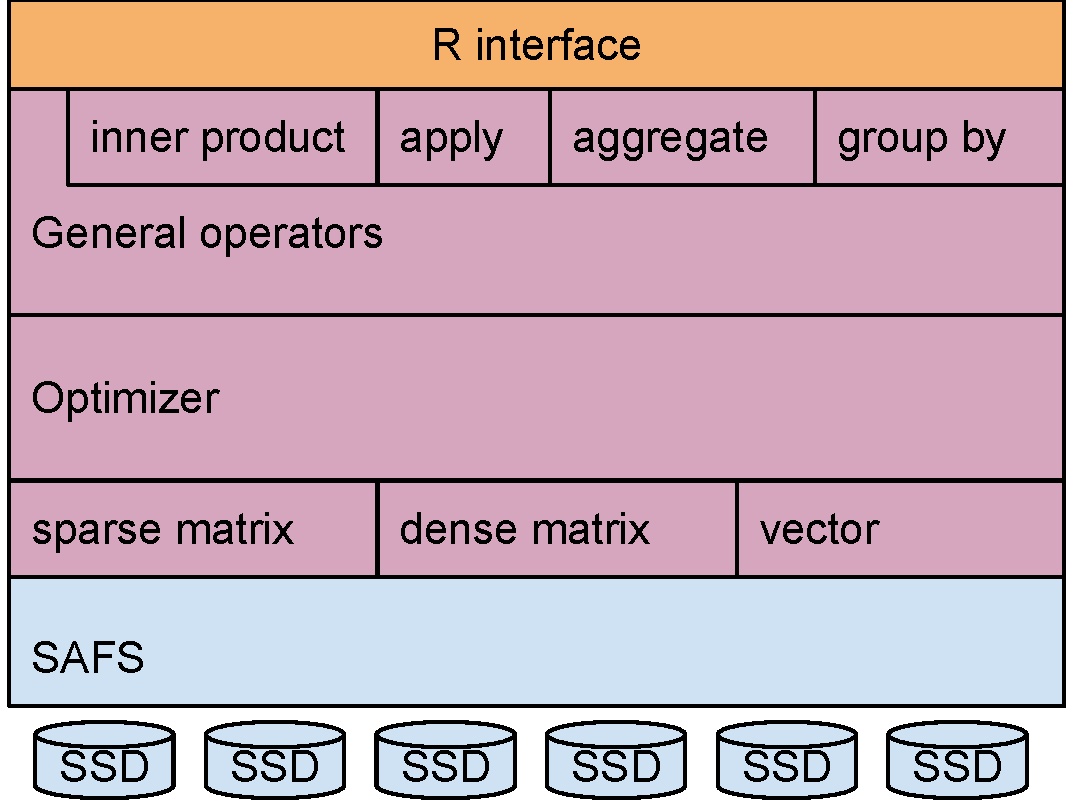
\includegraphics[scale=0.3]{./architecture.pdf}
\caption{The architecture of FlashMatrix.}
\label{fig:arch}
\end{figure}

\subsection{SAFS}

SAFS \cite{safs} is a user-space filesystem for a high-speed SSD array in
a NUMA (non-uniform memory architecture) machine. It is implemented as
a library and runs in the address space
of its application. It is deployed on top of the Linux native filesystem.
SAFS was originally designed for optimizing small I/O accesses. However,
sparse matrix multiplication and dense matrix operations
generate much fewer but much larger I/O. Therefore, we provide additional
optimizations to maximize sequential I/O throughput from a large SSD array.

The original SAFS has a dedicated I/O thread for each SSD. The I/O thread
accesses the SSD exclusively to avoid lock contention in the Linux kernel.
Application threads have to send I/O requests to one of the I/O threads
with message passing when accessing data from SSDs. It is necessary to have
one I/O thread for
an SSD when applications issue many small I/O accesses because processing
a large number of I/O accesses consumes a significant number of CPU cycles.
However, when the workload only has large I/O requests, each I/O request takes
much longer time to complete. As a result, the I/O threads are constantly put
into sleep while waiting for I/O and each I/O completion may suffer from
the latency of a thread context switch.

The latency of a thread context switch becomes noticeable on a high-speed SSD
array under a sequential I/O workload and it becomes critical to avoid thread
context switch to gain I/O performance. Therefore, instead of having an I/O
thread for each SSD, we use only a single I/O thread for each NUMA node, which
is responsible for all of the SSDs connected to the NUMA node. As such, an I/O
thread processes many more I/O requests to amortize the latency of a context
switch. Similarly, application threads communicate with I/O threads through
message passing when issuing I/O requests. If the computation in application
threads did not saturate CPU, SAFS would put the application threads into
sleep while they were waiting for I/O. This results in many thread context
switches and underutilization of both CPU and SSDs. To saturate I/O,
an application thread issues asynchronous I/O and poll for I/O to avoid thread
context switches after completing all computation available to it.

To better support access to many relatively small files simultaneously, SAFS
stripes data in a file across SSDs with a different striping order for each file.
This strategy stores data from multiple files evenly across SSDs and improves
I/O utialization. Due to the sequential I/O workload, FlashEigen stripes data
across SSDs with a large block size, on the order of megabytes, to increase I/O
throughput and potentially reduce write amplification on SSDs \cite{Tang15}.
Such a large block size may cause storage skew for small files
on a large SSD array if every file stripes data in the same order. Using
the same striping order for all files may also cause skew in I/O access.
Therefore, SAFS generates a random striping order for each file to evenly
distribute I/O among SSDs when a file is created. SAFS stores the striping
order with the file for future data retrieval.

\subsection{Data containers}
FlashMatrix supports both dense matrices and sparse matrices. FlashMatrix
represents a vector as a dense matrix. In this work, we mainly focus on
dense matrices. Some dense matrices are physically stored in memory or on SSDs,
but some are stored virtually. All elements in a matrix have the same primitive
type and FlashMatrix supports all primitive types in C/C++.
All matrices in FlashMatrix are immutable, which is required by lazy evaluation.
Each matrix has two identifiers: one for the matrix itself and the other for
the data in the matrix. When a matrix is cloned or transposed, the two matrices
have different matrix Ids but share the same matrix data Id.

\subsubsection{Tall-and-skinny matrix} \label{sec:tas_mat}

Tall-and-skinny (TAS) dense matrices commonly exist in many data mining
algorithms. As suggested by the name, these matrices have one of the dimensions
much larger than the other dimension (Figure \ref{fig:tas_mat}). A vector is
a special case of such a matrix. Many data matrices contain a large set of
data points with a relatively small number of features, so the shape of
the data matrices is usually tall and skinny. FlashMatrix can store TAS
matrices in memory and on SSDs and optimizes matrix operations specifically
for these matrices.

There also exist many wide-and-narrow matrices. For simplicity, we also refer
to wide-and-narrow matrices as a TAS matrix. 

\begin{figure}
	\centering
	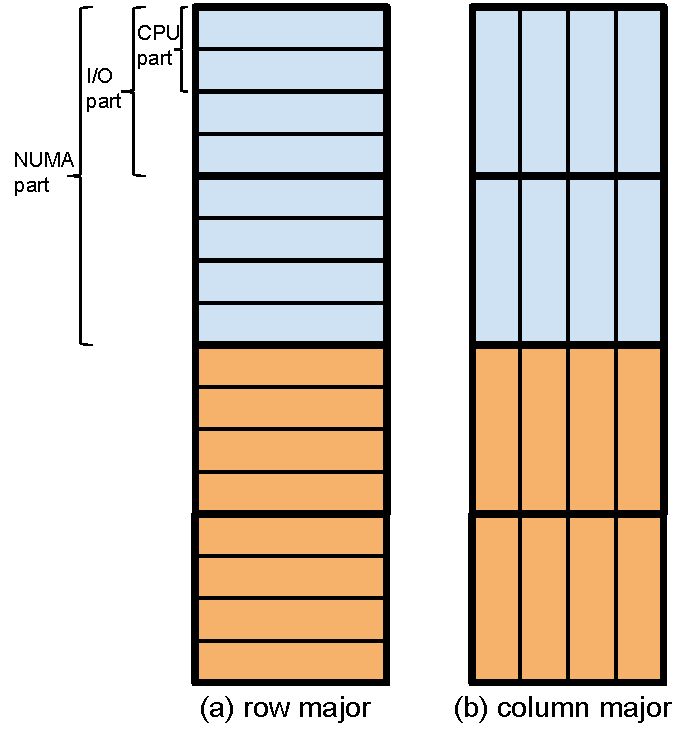
\includegraphics[scale=0.5]{./dense_matrix.pdf}
	\caption{The format of a tall-and-skinny dense matrix.}
	\label{fig:tas_mat}
\end{figure}

For parallelization and efficient data access, TAS matrices are partitioned
horizontally and in multiple levels (Figure \ref{fig:tas_mat}).
\begin{itemize}
\item NUMA-level partitioning: When a TAS
matrix is stored in memory, it is partitioned across NUMA nodes to achieve
data locality and fully utilize memory bandwidth. NUMA-level partitioning
tries to map partitions of different vectors/matrices involved in computation
to the same NUMA node to reduce inter-processor communication. As such,
the partition size (the number of rows in a partition) is a global parameter
and is not affected by the number of columns in a matrix. Having NUMA-level
partitioning helps us scale computation to a cluster.
\item I/O-level partitioning: Both in-memory and external-memory matrices have
I/O-level partitioning. A worker thread gets an I/O-level partition from each
matrix for computation and the partition size needs to be relatively large
(in the order of megabytes) to reduce overhead of retrieving a partition from
a matrix. The number of rows in an I/O-level partition is determined locally
and can be affected by the number of columns in a matrix.
All elements in an I/O-level partition are stored contiguously.
For an external-memory matrix, the I/O-level partition size determines an I/O
size. For an in-memory matrix, the partition size determines the size of
contiguous memory required in memory allocation (see Section \ref{sec:mem}).
\item CPU-level partitioning: We further split a matrix into smaller partitions
to reducing CPU cache misses when evaluating a sequence of matrix operations
(Section \ref{sec:lazy_eval}). For this level of partitioning, we keep
a partition small enough (in the order of kilobytes) to fit in CPU L1 cache.
The number of rows in a CPU-level partition is determined at runtime and
is affected by the number of columns in a matrix.
\end{itemize}
The number of rows in each level of partitioning is $2^i$

FlashMatrix supports both row-major and column-major matrices to avoid physical
data copy for some matrix operations such as matrix transpose. Due to
the partitioning scheme shown above, a column in a column-major TAS matrix
is not stored contiguously. FlashMatrix optimizes matrix operations for both
data layouts. The layout of a matrix is generally
determined by a FlashMatrix operation but can also be determined by users. 

If a dense matrix is stored on SSDs, it is stored in an SAFS file and we rely
on SAFS to stripe data across SSDs. SAFS stripes data in a file across SSDs
with a different striping order for each file.
This strategy stores data from multiple files evenly across SSDs and improves
I/O utilization. Due to the sequential I/O workload, FlashEigen stripes data
across SSDs with a large block size, on the order of megabytes, to increase I/O
throughput and potentially reduce write amplification on SSDs \cite{Tang15}.
Such a large block size may cause storage skew for small files
on a large SSD array if every file stripes data in the same order. Using
the same striping order for all files may also cause skew in I/O access.
Therefore, SAFS generates a random striping order for each file to evenly
distribute I/O among SSDs when a file is created. SAFS stores the striping
order with the file for future data retrieval.

\subsubsection{Virtual matrix} \label{virt_mat}
There are many cases that we do not need to store data of a matrix physically.
Instead, we use a special matrix that stores computation along with the input
of the computation, which we refer to as \textit{virtual matrix}. When a
\textit{virtual matrices} is used in computation, its data is generated on
the fly. A simple example is a matrix with all elements having the same value.
We never need to allocate memory for such a matrix physically.

\textit{Virtual matrices} becomes very useful in lazy evaluation (in Section
\ref{lazy_eval}).


With lazy evaluation, an operator outputs a special matrix to represent
the operation result and this special matrix does not store the actual data of
the operation result. Instead, it stores the computation and a reference to
the input matrices. We refer to these special matrices as
\textit{virtual matrices}.

\subsubsection{A group of dense matrices}
In some applications, we construct a group of dense matrices and always perform
operations on them together.

%\subsection{Basic operations} \label{sec:basic}
%create a data container

%data container conversion

%matrix operations: convert data layout and transpose.

%append an element to a vector can be implemented as physically appending the element
%to the vector. The result vector becomes the new vector, and the original vector
%becomes the sub-vector of the new vector.

\subsection{Generalized computation operations} \label{sec:generalized}
To enhance the flexibility and simplify the implementation, FlashMatrix only
provides a small set of generalized operators on vectors and matrices.
The current implementation has four generalized operators: \textit{inner product},
\textit{apply}, \textit{aggregation} and \textit{groupby}. Each operator
accepts user-defined functions (UDF). Like most of R functions, these operators
do not change data in the input data containers and each operation generates
a new data container.

FlashMatrix does not allow to access users to access individual elements.

\textit{Inner product} is a generalized matrix multiplication. It replaces
multiplication and addition in matrix multiplication with two user-defined
functions, respectively. As such, we can define many operations with inner
product. For example, we can use inner product to compute various pair-wise
distance matrics of vectors such as Euclidean distance \cite{euclidean} and
Hamming distance \cite{hamming}. We can also apply inner product to sparse
matrices to compute PageRank, belief propagation, etc.
Even though we can implement matrix multiplication with inner product,
FlashMatrix still relies on BLAS to implement matrix multiplicatoin for
float-point matrices to achieve speed and float-point precision required by
many numeric libraries such as the Trilinos eigensolver \cite{anasazi}.

\textit{Apply} is a generalized form of element-wise operations and has
multiple variants. The simplest form of \textit{apply}, denoted with
\textit{sapply}, is a generalized element-wise unary operation whose
UDF takes an element in a vector or a matrix at a time and outputs a value.
We can use it to implement unary operations such as negation, square root
or type casting of individual elements in a vector or a matrix. The second
form of \textit{apply}, denoted with \textit{mapply2}, is a generalized
element-wise binary operation whose UDF takes an element from each vector
or matrix and outputs a single value. We use it to implement many binary
matrix operations such as matrix addition and subtraction. The third form of
\textit{apply}, denoted by \textit{apply\_mat}, is a generalized row-wise or
column-wise operation whose UDF takes a row or a column at time and outputs
a vector of elements.

\textit{Aggregation} takes multiple elements and outputs a single element.
It has two forms on matrices. The first form, denoted by \textit{agg\_arr}
aggregates over all elements on a matrix. Operations such as summation and
maximum are special cases of the first form. The second form, denoted by
\textit{agg\_mat} aggregates over each individual row or column.
Row sum and column sum are special cases of the second form.

\textit{Groupby} takes a vector of elements along with a vector of categorical
values and invokes UDF on the elements associated with the same categorical
value. \textit{Groupby} also works on a matrix if we view a matrix as a vector
of vectors.

The function of some of the operators overlaps. For example, \textit{apply\_mat}
is a generalized form of \textit{agg\_mat}, but \textit{agg\_mat} can be
implemented more efficiently. Therefore, FlashMatrix provides both operators.

\subsection{Vectorized user-defined function}
UDF potentially introduces significant computation overhead. Traditionally,
UDF is applied to every individual element in a data container and, thus,
the computation on every element suffers from the large overhead of a function
call. Therefore, relying on UDF to implement commonly used vector and matrix
operations reduces the performance of the entire system significantly.
We need to highly optimize UDF to achieve the same performance as
the specialized matrix operations.

To amortize the overhead of function calls, all generalized operators take
vectorized user-defined functions (VUDF), which operates on an array of elements
instead of individual elements. The number of elements in an invocation of
VUDF determines how much overhead is amortized. However, too many elements
in one invocation potentially increase CPU cache misses when the computation
is constructed in a DAG shown in Section {}. For the elements of primitive
types, the number of elements in one invocation of VUDF can be as large as 1000,
which can still perfectly fit in the L1 CPU cache.

The generalized operators require multiple forms of VUDF. The first form takes
two arrays with the same number of elements and outputs an array of the same
length as the input arrays. The second form takes one array of elements and
a single element and outputs an array of the same length as the input array.
The first two forms are essential for binary operations such as
\textit{inner product} and \textit{mapply2} as well as \textit{agg\_mat} and
\textit{groupby\_mat}.
The third form takes an array of elements and outputs an array of the same
length, which is essential for \textit{sapply}.
The fourth form takes an array of elements and outputs a single element,
which is essential for \textit{aggregation}.

FlashMatrix has many commonly used VUDFs implemented in the framework by default.
These VUDFs wrap basic operations built in many programming languages and
libraries. For example, FlashMatrix provides arithmetic operations such as addition
and subtraction, relational operations such as equal to and less than, logical
operations such as logical AND and logical OR, as well as commonly used
math functions such as computing absolute values and square root. FlashMatrix
also provides a set of VUDFs to cast primitive element types. The built-in
binary operation usually needs to support three forms: form1, form2 and form3,
while the unary operation only needs to support form3. In addition, built-in
VUDFs also need to support different element types. Thus, each basic operation
supported by FlashMatrix has multiple VUDF implementations.

To reduce the number of VUDF implementations for different element types, form1
and form2 require the input elements to have the same type. If a generalized
operator gets two data containers with different element types, it first casts
the type of the elements in one container to match the element type of the other
container. Type casting follows the usual arithmetic conversions \cite{}
commonly seen in many programming languages. The type casting is performed
laziy and no additional data container is generated in type casting
(in Section \ref{sec:lazy_eval}).

For easier parallelization, generalized operators assume that VUDF is stateless.
Therefore, the generalized operators carry the mutable state of the computation.
However, VUDF can carry immutable values to simplify some implementations.

All different kinds of vectorized operators such as scatter and gather, aggregation.

We can use the basic VUDF to construct more complex VUDF for other generalized operators.


\subsection{Lazy evaluation} \label{sec:lazy_eval}
It is expensive to perform each matrix operation individually when matrices
become large. It causes significant I/O for
external-memory matrices and considerable memory allocation overhead for
in-memory matrices. Instead, FlashMatrix evaluates matrix operations lazily
and postpones evaluation whenever possible and uses a \textit{virtual matrix}
(in Section \ref{virt_mat}) to represent the output of a matrix operation.

There are multiple benefits with lazy evaluation. For external-memory matrices,
it reduces I/O, especially writes to SSDs. It is beneficial for in-memory
matrices because because it is expensive to allocate large memory chunks.
Another benefit is to enable operation fusion to improve parallelization
\cite{Ching12}. By taking special care of data movement in fused operations,
we minimize data movement between memory and CPU cache and achieve performance
close to manually-written C code.

The current implementation of FlashMatrix applies lazy evaluation to most of
the generalized operators. Lazy evaluation can be easily applied to
\textit{sapply} and \textit{mapply} because these two operations element-wise
operations. We also apply lazy evaluation to \textit{apply\_mat} and
\textit{agg\_mat} when these two operators runs on rows of a TAS matrix.
It is also applied to \textit{inner product} when \textit{inner product} runs
on a TAS matrix and a small matrix. In general, lazy evaluation is applied to
any generalized operator that outputs a large matrix.

To enable lazy evaluation, all matrices in FlashMatrix are immutable.
As such, \textit{virtual matrices} can generate the same result every time
they are materialized. As such, every matrix operation generates a new matrix
and a matrix is garbage collected when there are not any references to it.

\subsection{Matrix materialization}
Lazy evaluation postpones the actual computation of matrix operations,
but we eventually have to evaluate the matrix operations. Matrix materialization
is triggered when users materialize matrices or when users perform a matrix
operation that cannot be lazily evaluated. We need to materialize matrices
with caution because lazy evaluation may have the cost of increasing
computation or even increase reads from SSDs if a \textit{virtual matrix}.
is materialized multiple times. When materializing a \textit{virtual matrix},
we should also keep data in the CPU cache as much as possible to improve
performance.

\begin{figure}
	\centering
	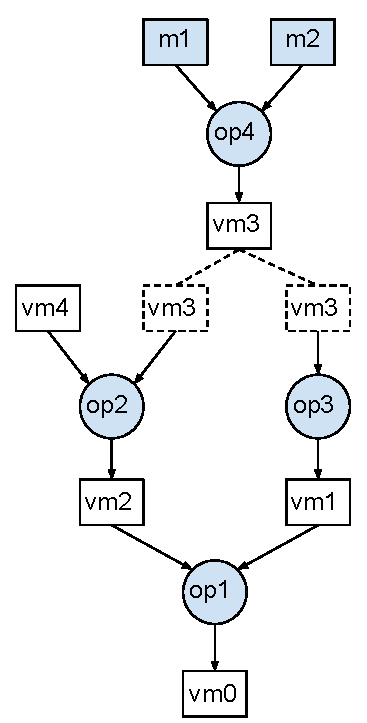
\includegraphics[scale=0.5]{./op_tree.pdf}
	\caption{An operation tree.}
	\label{fig:op_tree}
\end{figure}

We use an operation tree to represent computation in a \textit{virtual matrix}
(Figure \ref{fig:op_tree}) instead of directed acyclic graph (DAG) \cite{}
to simplify evaluation. As such, we can evaluate a \textit{virtual matrix}
recursively. When representing computation as a tree, we need to take special
care of the matrices shared by multiple operators. There are two types of nodes
in an operation tree: an operation node (shown as a cycle) and a matrix node
(shown as a rectangle). A matrix node represents a TAS matrix. Small matrices
or scalar variables are kept as computation state in operation nodes. A generalized
operator
takes one or two matrices as input matrices, so an operation node has at most two
children nodes. A generalized operator outputs at most one \textit{virtual matrix},
so an operation node has at most one parent node. The solid arrows connect
operation nodes with matrix nodes and indicate data flow in computation.
The node \textit{vm3} in Figure \ref{fig:op_tree} shows a case that a matrix
is shared by multiple generalized operators as an input matrix.

All TAS matrices in an operation tree are partitioned horizontally to parallelize
evaluation of an operation tree. All TAS matrices in an operation tree have to
have the same height so that each partition has the same height and we can
materialize each partation independantly. All matrices are split into I/O-level
partitions to balance the overhead of accessing a partition, parallelization
skew and memory consumption. When there are external-memory matrices in
an operation tree, we use the I/O-level partition size of external-memory
matrices for parallelization to avoid a partition from being accessed multiple
times.
%a global dispatcher. from top to bottom.

To reduce data movement among CPU cache, main memory and SSDs, FlashMatrix is
capable of three levels of matrix materialization to handle different cases.
\begin{itemize}
\item For a matrix used only once, a worker thread further splits an I/O-level
	partition into CPU-level partitions (Section \ref{sec:tas_mat}) and
	materializes one CPU-level partition at a time. When a CPU-level partition
	is materialized, it is passed to the subsequent operation in the operation
	tree. Because a CPU-level partition is small enough to fit in the CPU cache,
	the materialized partitions stay in the CPU cache throughout the operation
	evaluation on the partition range. To keep data in CPU cache as long as possible,
	we reuse the memory buffers to reduce the number of memory buffers used
	in the computation and avoid CPU cache polution.
\item For a matrix that only appears in one operation tree but are shared by
	multiple operators, a worker thread cache a materialized I/O-level partition
	locally when the partition is materialized. Because we parallelize matrix
	operations in the I/O-level partitions, the cached partition will be reused
	when the worker thread meets the same matrix again. A worker thread only needs
	to cache one partition from a matrix at a time, so it can use the matrix data
	Id to identify the partition. As such, even if we encounters the transpose
	of the matrix, we can still find the right partition in the local cache.
\item We require full materialization of a \textit{virtual matrix}
	when it is used in multiple sequence of matrix operations. As such,
	Users can explicitly materialize a \textit{virtual matrix}. In some cases,
	it is desirable to fully materialize an intermediate matrix in a matrix
	operation sequence. Therefore, users can also set a flag on a
	\textit{virtual matrix} to inform FlashMatrix to materialize it.
\end{itemize}

\subsection{Memory management} \label{sec:mem}
It is expensive to allocate large memory. Linux uses \textit{mmap} to allocate
large memory in the order of megabytes. Linux relies on page fault to populate 
the memory allocated by \textit{mmap} with physical pages when they are used
for the first time.
The overhead becomes considerable when we allocate and deallocate large memory
constantly. Frequent page fault also prevents computation from fully utilizing
CPUs in a large parallel machine. Furthermore, memory allocation occurs frequently
in FlashMatrix because all data containers are immutable due to lazy evaluation
(Section \ref{sec:lazy_eval}). As such, we manage large memory allocation
ourselves to reduce such overhead. We need large memory allocation for creating
in-memory vectors and matrices as well as allocating memory buffers for
computation.

special memory allocation for constructing an in-memory matrix and keeping part
of a matrix during computation.

\begin{figure}
	\centering
	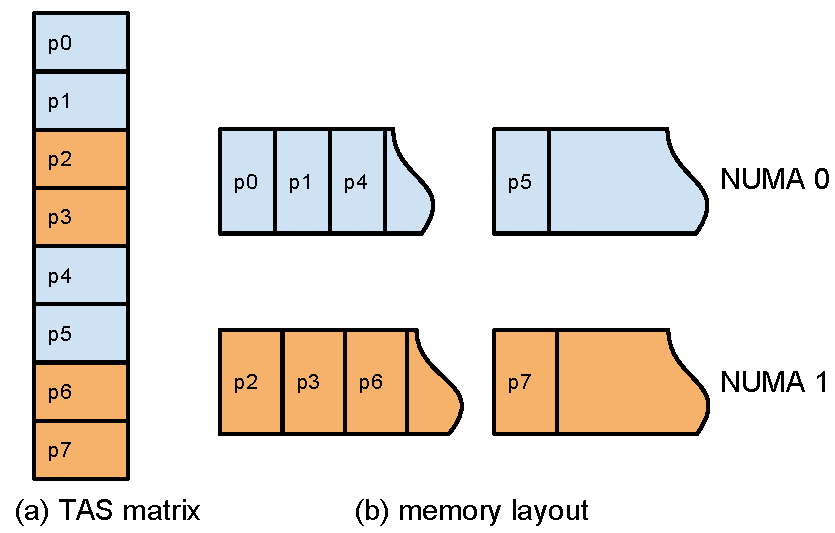
\includegraphics[scale=0.5]{./matrix_mem.pdf}
	\caption{Memory layout of a tall-and-skinny dense matrix.}
	\label{fig:mat_mem}
\end{figure}

To reduce the overhead of memory allocation with \textit{mmap}, we recycle
memory allocated for in-memory vectors and matrices. Instead of deallocating
memory used
by other containers when the containers are destroyed, we retain the memory
and assign them to the next created containers. To help recycle memory, we
allocate fixed-size memory chunks for a vector or a matrix. The size of
a memory chunk is a global parameter and is the same for all vectors and
matrices. As such, memory chunks allocated for a matrix can be used by a vector
or a matrix with a totally different shape. We perform matrix operations on
I/O-level partitions and only require an I/O-level partition to be stored in
contiguous memory. Therefore, we can store a matrix in memory chunks and
perform computation on it, as long as a fixed-size memory chunk is sufficient
to store an I/O-level partition. In practice, the memory chunk size may
not be divisible by the I/O-level partition size. Therefore, the memory chunk
size needs to be much larger than the I/O-level partition size to increase
memory utilization.

We further maintain per-thread memory buffer pools to store data read from
SSDs or materialized from a virtual matrix. These memory buffers need to be
the same size as I/O-level partitions, which is in the order of megabytes
to maximize I/O throughput of an SSD. Due to asynchronous I/O, a worker thread
needs to allocate a small number of memory buffers for each vector or matrix
during computation. Because all partitions in a vector or a matrix have
the same size, the memory buffers are reused for processing other partitions
of vectors or matrices.

\subsection{Implementation details}

Avoid allocating memory in one thread and deallocating in another thread.

\subsection{Integration with R}

FlashMatrix provides an R extension called FlashR to seamlessly integrate with
R and power R for large-scale data mining. FlashR provides wrapper functions
for each of the generalized operators
in FlashMatrix. In addition, we implement many commonly used R functions with
the generalized operators to provide R users a familiar programming environment
while the underlying optimizer in FlashMatrix merges operations and
automatically parallelizes complex algorithms written in R.

The current implementation provides a large set of built-in VUDFs in FlashR.
Users are able to implement many R functions with these built-in VUDFs.
Users can also implement their own VUDFs in C/C++ and load to R to further
extend the capability of FlashR.

Garbage collection of vectors and matrices.

implement more VUDF and register them.

The full set of operations supported in R.
Matrix construction,
Matrix conversion,

\subsection{Applications}

We implement a few well-known data mining algorithms to demonstrate
the flexibility and the performance of FlashMatrix. All of the algorithms
can be expressed with a set of vector and matrix operations. We implement
all of them with its R interface.

KMeans is one of top 10 data mining algorithms identified by the IEEE
International Conference on Data Mining (ICDM) \cite{top10}.

\begin{figure}[t]
%\begin{lstlisting}
\begin{minted}[mathescape,
		fontsize=\scriptsize,
		frame=single,
]{r}
# calculate the new centers by averaging data pointers
# in a cluster.
cal.centers <- function(data, parts) {
	n <- dim(data)[1]
	one <- rep.int(1, n)
	sizes <- groupby(one, parts, sum)
	centers <- groupby(data, parts, sum)
	centers <- diag(1/sizes) %*% centers
}

#initialize centers
n <- dim(data)[1]
m <- dim(data)[2]
rand.parts <- floor(runif(n, min=1, max=K+1))
new.centers <- cal.centers(data, rand.parts)
centers <- matrix(rep.int(0, K * m), K, m)

while (sum(centers == new.centers) == length(centers)) {
	centers <- new.centers
	m <- inner.prod(data, t(centers), dist, add)
	# calculate the new center of each data pointer.
	dp.centers <- apply(m, 1, which.min)
	new.centers <- cal.centers(data, dp.centers)
}
\end{minted}
%\end{lstlisting}
\vspace{-5pt}
\caption{The implementation of KMeans.}
\label{fig:kmeans}
\end{figure}

%TODO each KMeans iteration only needs to read the entire data matrix once.
